\documentclass{article}
\usepackage{graphicx} % Required for inserting images
%Math Stuff
\usepackage{amsmath} % many display options for math modes and such (VERY IMPORTANT)
%\usepackage{physics} % useful math symbols and macros (VERY IMPORTANT)
\usepackage{amssymb} % heck ton of math symbols and fonts (VERY IMPORTANT)
\usepackage{amsfonts} % Additional fonts, math symbols, and options for existing fonts (IMPORTANT)
\usepackage{mathtools} % lots of cool mathtools oh wait that is the name (IMPORTANT)
\usepackage{siunitx} % allows you to quickly define units within math mode (IMPORTANT)
\usepackage{array} % allows you to write piece-wise functions, matrices, and other cool things (IMPORTANT)
\usepackage{txfonts} % defines times new roman as default text font and provides supporting math symbols
\usepackage{braket} % allows the use of detailed Dirac braket notation
\usepackage{cancel} % used to cancel terms (with X or diagonal line) while writing math (useful for assignments)
\usepackage{ulem} % underlines, typewriter font (for comp sci somewhat), and striking out (required for cancel package)
\usepackage{empheq} %Extension of amsmath for boxing equations or answers


%Formatting Stuff
\usepackage[utf8]{inputenc} % the typesetting rules
\usepackage[left = 22mm, right = 22mm]{geometry} % flexible and easy interface to change page dimensions
\usepackage{graphicx} % provides additional options for figures
\usepackage{float} % allows you to tell latex no really I want the figure HERE (with H)
\usepackage{color} % provides coloring capabilities to everything
\usepackage{fancyhdr} % making fancy headers (obviously)
\usepackage{changepage} % allows to change page formatting in the middle of a document (rather than the same throughout) 
\usepackage{enumitem} % better control over enumerate and itemize
\usepackage[labelfont=bf]{caption} % altering options for captions
\usepackage{sidecap} % allows sideways captions for figures and tables
\usepackage{soul,xcolor} % can enhance striking, underlining, and highlighting (in non-math mode)

\usepackage{afterpage}
\newcommand\blankpage{%
    \null
    \thispagestyle{empty}%
    \newpage}
\usepackage[hidelinks]{hyperref}

\title{Trigger System Start Up Procedure}
\author{Gabby Gelinas}
\date{Updated August 2, 2024}

\begin{document}

\maketitle

\section*{Cabling}
The cabling system for all boards is identical. Please see the image provided. It is important to note that there are three identical gold inputs: one alone and two in a pair. Starting from the outermost input of the pair, their inputs are: calibration pulse, analog signal for the lower numbered board, analog signal to the higher numbered board.

\begin{figure}[H]
    \centering
    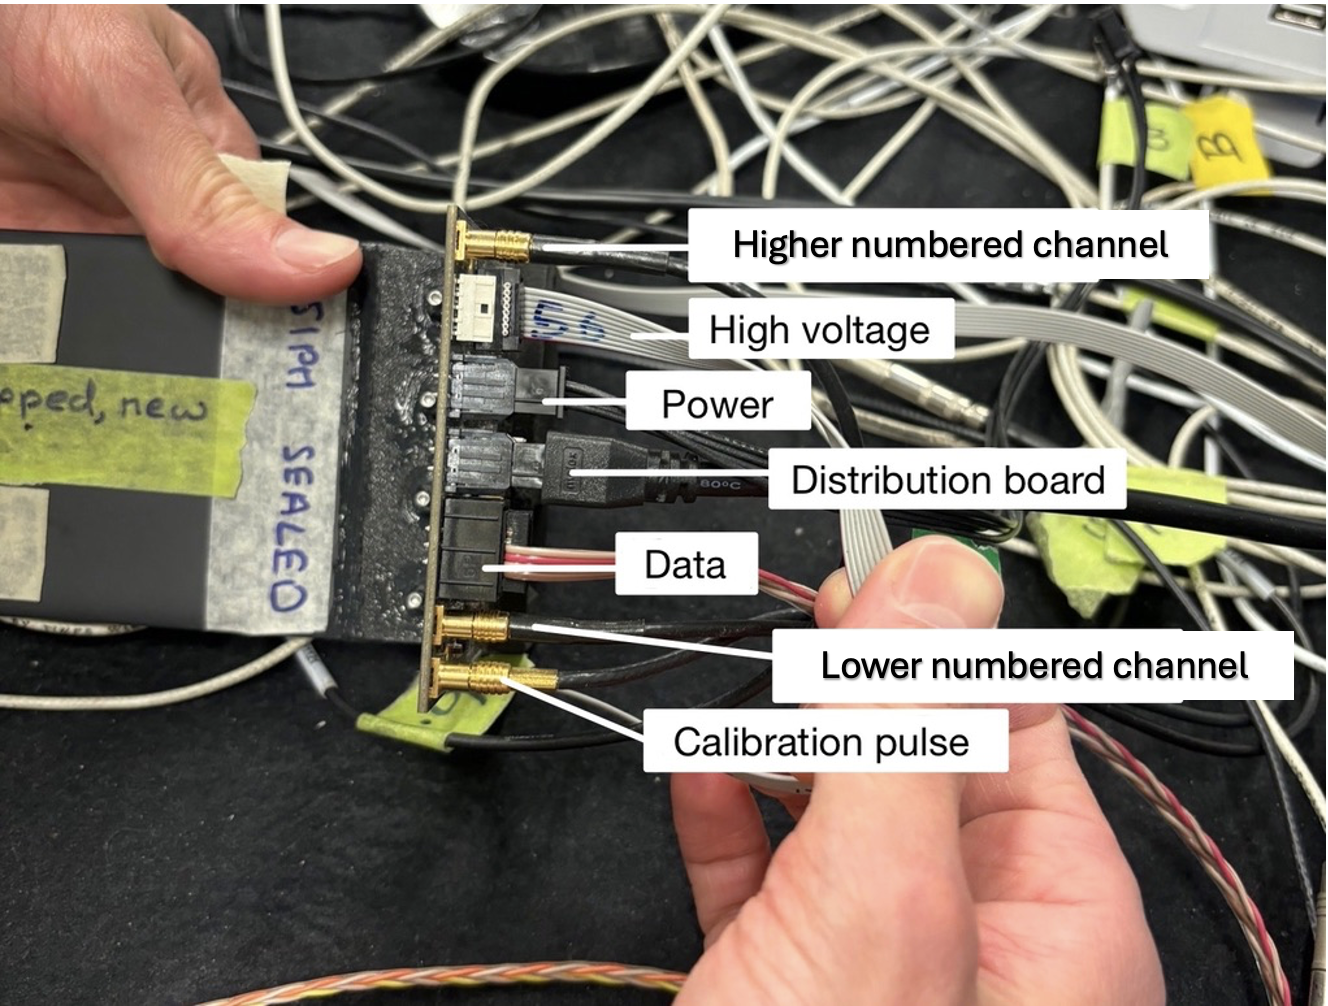
\includegraphics[scale=0.5]{boardPorts.png}
    \caption{Labeled cabling example for one of the PCBs attached to the end of a scintillator.}
    \label{fig:enter-label}
\end{figure}


\section*{Set Up and Starting a Run}

\begin{enumerate}
    \item Open the DAQ status page at \url{https://daq17.triumf.ca} and sign into midas when prompted. Username is `1eanpk\_dl", password is ``1eanpk\_dl".
    \item This will open to the midas status page. You may get a big red message saying “Alarm: program fedldb is not running”. This is ok, the distribution just isn't on yet.
    \begin{itemize}
        \item Fedldb means “front end DarkLight distribution board”.
    \end{itemize}
    \item \textbf{Turn on low voltage} using the power supply on the table with the green tape on it. Just press the power button, do not turn any knobs. 
    \begin{itemize}
        \item It should settle at 6 V, the ideal values are written on the power supply. You should see zero current. The boards aren't drawing any because they aren't turned on. You haven't turned the distribution board on yet so it isn't sending power to the boards.
    \end{itemize}
    \item Turn the \textbf{fans} on by turning on the power strip labeled “fans”.
    \item Open the “programs” tab. \textbf{Start fechrono02} (the choronobox), and \textbf{fedldb} (the distribution board).
    \item Once the fedldb is running (green in “programs” tab) you can go back to the status page and press rest on the alarm and it should go away.
    \item From the side panel, open ``DLDB" to control the distribution board. Make sure all boards you are going to use are set to ``enabled". You can change this in "settings" beside "ODB actions"
    \item Click \textbf{Init} then \textbf{all on} to start sending low voltage power to the SiPMs. 
    \begin{itemize}
        \item You know that it worked if you see current being drawn on the low voltage power supply.
    \end{itemize}
    \item \textbf{Set the threshold}. The threshold (thr) is set as a hex value. Setting it as 4096 gives you 80 mV, please see the overleaf for more values. Press \textbf{“write thresholds”} on the main DLDB page for this change to take effect. If you are not changing the threshold, still press the ``write thresholds" button.
    \item \textbf{Turn high voltage on}. Flip the on switch, then press in the green output button, then slowly turn the voltage knob up to 10ish V. 
    \begin{itemize}
        \item If “vbias demand” in DLDB is set to 0, none of this voltage will actually be seen by the boards.
    \end{itemize}
    \item In the DLDB tab, open “settings”. \textbf{Adjust each voltage under ``vbias demand"} to what you need. If unsure, 53.9 V is good. 
    \begin{itemize}
        \item Press \textbf{“vbias on”} to have your vbias demand changes take effect and send high voltage power to the boards.
        \item vbias\_dac converts the number you set in vbias demand to what controls the amount of voltage that goes through.
        \item The distribution board dissipates 5-10 V so you will see a discrepancy between what you set on the high voltage power supply and the value in “vbias\_meas”. You will need to set the high voltage power supply higher than what you need because of this.
        \item If you run into problems here like vbias\_meas not being within 5ish V of what you set it to, go back to the programs tab and stop fedldb and restart it.
    \end{itemize}
    \item Continue to \textbf{increase the high voltage supplied} by turning the knob on the power supply.
    \begin{itemize}
        \item Once reaching approximate the voltage you demanded at the boards, increasing the voltage at the high voltage power supply will not increase vbias\_meas since the distribution board will not send more to the boards.
    \end{itemize}
    \item To get live updated plots, go the “history” tab on the side panel.
    \begin{itemize}
        \item Rates should be around 1-10 counts/second. If they are significantly higher it means you haven’t set the threshold.
        \item Temperatures across all four boards should be similar, though some variation is normal due to fan positioning and differences in fan power.
        \item Vbias should match what you saw in the DLDB tab.
        \item dldb\_vbias is the voltage at the distribution board.
        \item dldb\_ibias is the current on the distribution board in mA.
        \item As of April 23, 2024, dldb\_vbias and dldb\_ibias are not properly calibrated.
        \item To zoom in, drag on the axis. To zoom out, press control r. Every time you change the zoom the plot pauses. Play play button on the right to resume.
    \end{itemize}
    \item You are now ready to \textbf{start a run}. On the status page and press “start”. \textbf{Add a descriptive comment}. Generally, the comment includes the type of run (comics, pulsar/calibration, and source), the threshold, the vbias on each of the boards, what mask you are using, and any other notes like if there’s a gap between the paddles or if you introduced a new board. Press start and your run has begun!
    \begin{itemize}
        \item Masks are data filters in either the TDC or the FPGA. It sets what data is recorded (paddle coincidence - 0x40fe, top and bottom coincidence - 0x40f0, all hits - no mask)
    \end{itemize}
    \item During a run you can use the “rootana” tab on the side bar to view the root plots in live time. This tab only works when there is a run going. You can’t look at the last run if it has already ended. You will need to open the root file yourself to do that.
\end{enumerate}

\section*{Turning the System Off}
\begin{enumerate}
    \item On the status page, stop the run.
    \item On DLDB page, turn vbias off.
    \item Turn the high voltage down to 40 V on the power supply, then press the output button, the turn it off.
    \item On the DLDB page, turn SIPM power off by pressing ``all off".
    \item In “programs” stop fedldb since no power is going to the distribution board anymore.
    \item Turn off the low voltage power supply by just pressing the button, do not touch any knobs.
    \item Turn the switch for the fans off.
\end{enumerate}

You only need to turn everything off if you are re-cabling. If you just aren't taking data at the moment, leave everything on so someone else has the option to start a run remotely.

% ADD SOMETHING ABOUT HOW CHANNELS MUST SAY "YES" TO BE ENABLED

\end{document}
